
\documentclass[11pt,preprint]{aastex}

%compact captions %%%%%%%%%%%%%%%%%%%%%%%%%%%%%%%%%%%%%%%%%%%%%%%%%%%
%\usepackage[font=small,labelfont=bf, textfont=it, justification=justified]{caption}
%\DeclareCaptionFormat{ruleformat}{\baselineskip0.2cm\hrulefill\\\noindent#1#2#3{\hrulefill}}
%\captionsetup[figure]{format=ruleformat}
\setlength{\textfloatsep}{0pt}
%\setlength{\abovecaptionskip}{-10pt}
\setlength{\floatsep}{2pt}

\usepackage{verbatim}
\usepackage{rotating}
\usepackage{lscape}
\usepackage{subfigure}
\usepackage{natbib}
\usepackage{arydshln}

\usepackage[colorlinks=true, linkcolor=blue, urlcolor=blue, citecolor=blue, pdftex, bookmarks=true, linktocpage=true, hyperindex=true]{hyperref}
\usepackage{breakurl}

\providecommand{\xxxx}{{\color{red} ~XXXX~}}
\providecommand{\xsede}{XSEDE~}
\providecommand{\eg}{e.g.,~}
\providecommand{\ie}{\textit{i.e.},~}
\providecommand{\msun}{M$_\odot$~}

\newlength\tindent
\setlength{\tindent}{\parindent}
\setlength{\parindent}{0pt}
\renewcommand{\indent}{\hspace*{\tindent}}

\begin{document}


\section{ Computational Methodology and Algorithms}
We use the Flexible Stellar Population Synthesis \citep[FSPS;][]{fspsI, fspsIII} code for computing the spectrum and photometry of stellar populations, combined with the \texttt{emcee} code for MCMC sampling of posterior probability function to infer the physical parameters of observed stellar clusters.  Parallelization is achieved during the MCMC sampling.

\subsection{FSPS}
FSPS is a Fortran code used to generate flexible, state-of-the-art models of the spectra of stellar populations.  It uses tabulated stellar isochrones and a user defined initial mass function (IMF) to calculate the number of stars with different physical properties.  Tabulated spectra are then combined with weighting by the relative number of stars of each spectral type.  In a separate step dust extinction is applied, and the spectrum is convolved with a Gaussian to model the spectrograph resolution.  All tables are loaded into memory at the start of the code, so that there is no I/O during code execution.

We use lightweight Python bindings to the Fortran code, generated with \texttt{f2py}.  We have tested that the Python bindings do not add significant computational time, which is dominated by interpolation and integration within the FSPS Fortran code.  On Stampede model generation takes approximately 4s on a single core, and FSPS model generation thus dominates the computational time required for calculation of posterior probabilities and the code run-time in general. Significant efforts have been made to speed up FSPS as much as possible.

\subsection{Flexible calibration model}
For real data it is necessary to model the uncertain spectral calibration.  To do this we use a polynomial combined with a Gaussian Process \citep[e.g.,][]{RW} to model the covariance between the fluxes at nearby wavelengths.  Inversion of the covariance matrix is accomplished via \texttt{Scipy}'s Cholesky decomposition algorithms, which in turn use the Intel MKL library.

\subsection{MCMC sampling: \texttt{emcee}}
\label{sec:emcee}
\texttt{emcee} is a Python implementation of the affine-invariant ensemble MCMC sampling scheme of \cite{goodman_weare}.  It opertes via an ensemble of ``walkers'' that move in the model parameter space, where the new parameter position for a each walker is based on the posterior probability of the parameters at other walker positions.   This process is iterated until the distribution of walker positions converges to a stable distribution, which is an approximation to the $N_{parameters}$-dimensional posterior probability distribution. The number of iterations, $N_{iterations}$, required depends on the initial positions of the walkers, the number of walkers $N_{walkers}$, and the quality of the data.  The total number of posterior probability or likelihood evalutions is $N_{likelihood} = N_{walkers} \times N_{iterations}$.

In the \texttt{emcee} implementation, at each iteration the ensemble of walkers is split in 2 equal subsamples. The posterior probabilities at the positions of the walkers in one subsample are computed in parallel, and are then used to propose new parameter positions for the other subsample. Using \texttt{mpi4py}, MPI communication of parameter position vectors and scalar posterior probabilities between cores takes place twice per iteration. Since the computation of the posterior probabilities dominates the total run time of the code, large speedups can be obtained by increasing the number of cores up to $N_{walkers}/2 + 1$.  

On Stampede, we have found that, for mock data and for $N_{walkers}$ between $\sim$126 and 510, increasing $N_{walkers}$ (and thus the number of cores that can be used efficiently) also decreases the number of iterations required before the distribution of walkers converges.  That is, for 2 times as many walkers, the number of iterations required for convergence decreases by at least a factor of 2, thus maintaining or even decreasing the total problem size.  We are currently investigating the optimal number of walkers - at very low numbers of iterations ($\sim 100$) we expect the distribution to still be evolving even for exceedingly large numbers of walkers (and cores).

The stored walker positions are transferred to local servers to run our custom diagnostic and visualization software.  
In cases where the walkers in the sampler have not converged to a stationary distribution in parameter space, we can restart the sampler from the last ensemble of positions, thus taking advantage of previous computations.  
We are investigating techniques for robust online assessment of sampler convergence.


\subsubsection{Load Balancing}
The \texttt{emcee} offers the option of load balancing the computation of the posterior probabilities when there are more than twice as many walkers as there are cores.  However, we have found that the time for the posterior probability computation does not vary by more than 10\%, and cannot be predicted easily. Thus load balancing does not provide a significant speedup. 

If the number of walkers is not a $K>2$ integer multiple of $N_{cores}-1$ then some processors will not be utilized effictively.  In our code the number of walkers is determined at run time from the number of processors to insure maximum efficiency.

\section{Benchmarks and Scaling}
In our tests the \texttt{emcee} algorithm scales well with the number of cores as long as the number of walkers is an integer multiple of the number of cores minus one.  This is because the work is completely dominated by the calculation of the of the posterior probabilites, which requires both generation of the stellar population model and inversion of $\sim 2\mbox{k} \times 2\mbox{k}$ matrices. A large number of walkers also decreases the number of iterations required for convergence, keeping the total problem size fixed (or even making it smaller)

In Figure \ref{fig:scaling} we show scaling results for runs on Stampede.  This Figure shows the number of total number of likelihood calculations made, $N_{likelihood}$, divided by the wall time required as a function of the number of cores for several test runs.  These test runs used simplified, lower-resolution spectral models.  For some of them we did not perform matrix inversions for the likelihood evaluation, resulting in approximate $2 \times$ faster individual likelihood calculations.  The number of likelihoods evaluated per second scales almost exactly with the number of cores, for a variety of total problem sizes, $N_{likelihood}$.

\begin{figure}
\begin{center}
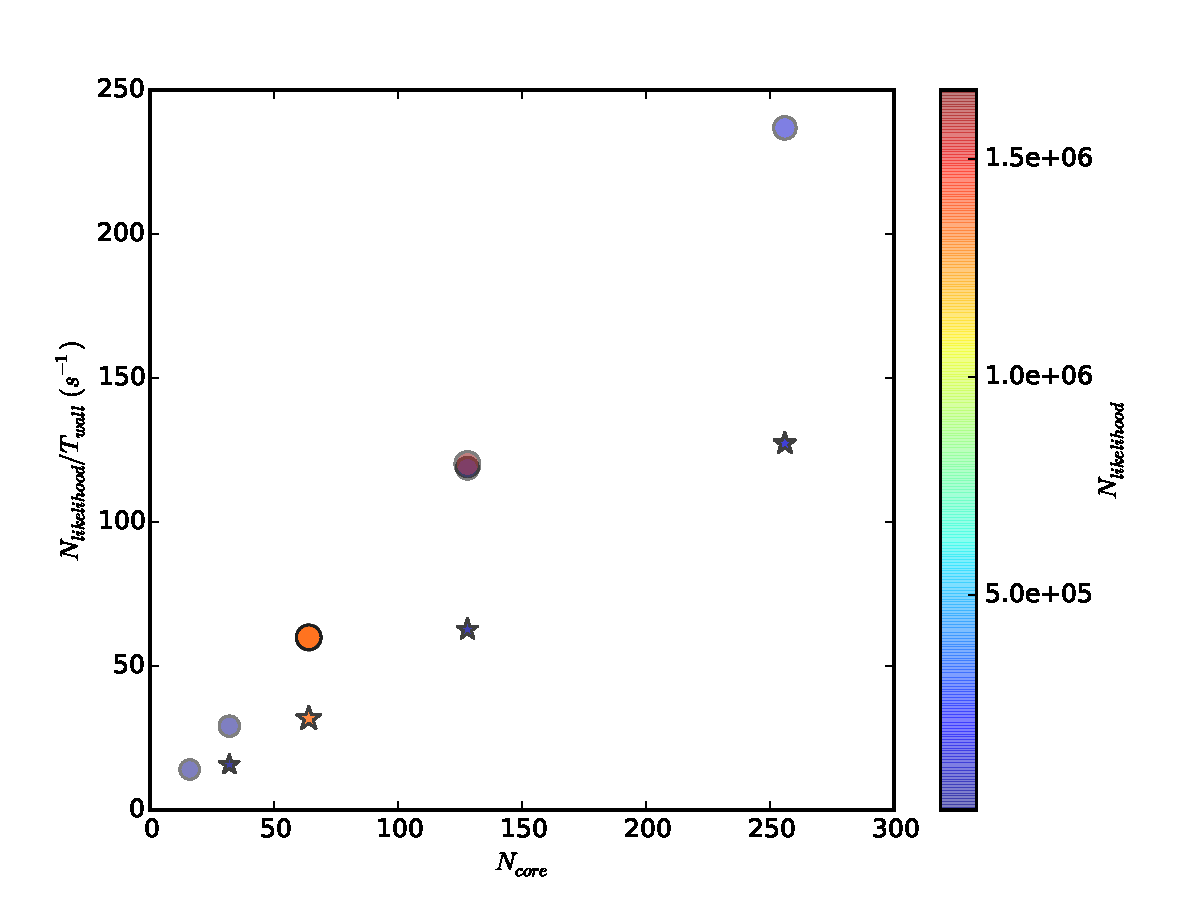
\includegraphics[width=0.8\textwidth]{efficiency.pdf}
\caption{Stampede scaling tests. The total number of likelihood calls divided by the total runtime is plotted as a function of the number of cores.  The symbol color and size encodes the total problem size, defined as the total number of likelihood calls requested.  Circles are for a restricted model with fast spectral model generation and no matrix inversions, stars are for the fast model generation but with matrix inversion for the Gaussian Process calibration model, resulting in longer times for each likelihood call. \label{fig:scaling}}
\end{center}
\end{figure}
\begin{thebibliography}

\bibitem[{{Conroy} {et~al.}(2009)}]{fspsI} 
Conroy, C., Gunn, J.~E., \& White, M.\ 2009, \apj, 699, 486 

\bibitem[{{Conroy} \& {Gunn}(2010)}]{fspsIII} 
Conroy, C., \& Gunn, J.~E.\ 2010, \apj, 712, 833 

\bibitem[{{Foreman-Mackey} {et~al.}(2013)}]{emcee} 
Foreman-Mackey, D., Hogg, D.~W., Lang, D., \& Goodman, J. 2013, \pasp, 125, 306 

\bibitem[{{Goodman} \& {Weare}(2010)}]{goodman_weare} 
Goodman, J., \& Weare,  J. 2010, Commun. Appl. Math. Comput. Sci., 5, 65

\bibitem[{{Rasmussen} \& {Williams}(2006)}]{RW}
Rasmussen, C.E., \& Williams, C.W., the MIT Press, 2006

\end{thebibliography}

\end{document}